\documentclass[12pt,xcolor=svgnames]{beamer}
\usepackage{dsfont,natbib,setspace}
\mode<presentation>

% replaces beamer foot with simple page number
\setbeamertemplate{navigation symbols}{}
\setbeamertemplate{footline}{
  \vspace{-1.5cm}
  \raisebox{10pt}{\makebox[\paperwidth]{\hfill\makebox[20pt]{\color{gray}\scriptsize\insertpagenumber}}}}

% colors
\newcommand{\bk}{\color{black}}
\newcommand{\rd}{\color{red}}
\newcommand{\fg}{\color{ForestGreen}}
\newcommand{\mar}{\color{Maroon}}
\newcommand{\org}{\color{Orange}}
\newcommand{\bl}{\color{blue}}
\newcommand{\gr}{\color{gray}}
\newcommand{\theme}{\color{FireBrick}}
\newcommand{\fb}{\color{FireBrick}}
\newcommand{\hlf}{\setstretch{1}}

% common math markups
\newcommand{\bs}[1]{\boldsymbol{#1}}
\newcommand{\mc}[1]{\mathcal{#1}}
\newcommand{\mr}[1]{\mathrm{#1}}
\newcommand{\bm}[1]{\mbox{\boldmath $#1$}}
\newcommand{\mb}[1]{\mathbf{#1}}
\newcommand{\ds}[1]{\mathds{#1}}

% spacing and style shorthan
\newcommand{\sk}{\vspace{.4cm}}
\newcommand{\nochap}{\vspace{0.5cm}}
\newcommand{\nsk}{\vspace{-.4cm}}
\newcommand{\chap}[1]{{\theme \Large \bf #1} \sk}
\newcommand{\R}[1]{{\bl\tt #1}}
\newcommand{\til}{{\footnotesize$\bs{\stackrel{\sim}{}}$ }}

% specific stats markups for this doc
\newcommand{\E}{\ds{E}}
\newcommand{\Reals}{\ds{R}}
\newcommand{\pr}{\text{Pr}}
\newcommand{\var}{\text{var}}
\newcommand{\cov}{\text{cov}}
\newcommand{\mT}{\mc{T}}
\newcommand{\GP}{\mc{GP}}
\newcommand{\iidsim}{\stackrel{\mathrm{iid}}{\sim}}
\newcommand{\indsim}{\stackrel{\mathrm{ind}}{\sim}}
\newcommand{\mN}{\mc{N}}
\newcommand{\mL}{\mc{L}}


\begin{document}

{ \usebackgroundtemplate{}%\includegraphics[height=\paperheight]{phoenix}}
\thispagestyle{empty}
\setcounter{page}{0}

%first review sampling distributions, then talk about sampling distributions for the OLS parameters, then prediction
%right now it goes prediction, review, OLS params, prediction

\title{\theme \Large \vskip 0.5cm
{\bf VectorBiTE Training 2018 \\ Methods Workshop}\\
\bigskip
\bf {\sf \gr Basics of Probability and Statistics}}

\author{
\begin{center}

\includegraphics[scale=0.15,trim=10 10 0 150]{VB_logo}
\end{center}
\texttt{\rd\small www.vectorbite.org}
%Normal distribution, distribution of the sample mean, \\
%Central Limit Theorem, Confidence Intervals
%and Method of Moments
%Review of sampling distributions
%Parameter estimation, sampling distributions,\\ 
%coefficient testing, and prediction intervals\\
%\vskip 1cm {\bf Leah R.~Johnson}\\ 
%{\org Virginia Tech}, Statistcs\\
%  \vskip .5cm \texttt{\rd\small leah.johnson-gramacy.com/QED/teaching}
}
\date{}
\maketitle 
}

% doc spacing
\setstretch{1.1}


\begin{frame}
\chap{Assumed Background} 

I assume that you've seen most of this before. This material is covered in more depth in the assigned reading. In particular, I expect that you know:

\begin{itemize}
\item axioms of probability and their consequences.
\item conditional probability and Bayes theorem
\item definition of a random variable (discrete and continuous)
\item the idea of a probability distribution and likelihood
\end{itemize}

We'll do a VERY fast review of these and do some practice exercises, including with {\sf R}.

Note -- We won't review confidence intervals, p-values, the central limit theorem, etc.

\end{frame}

\begin{frame}
\chap{Some probability notation} 

We have a {\bl set}, $S$ of all possible events. Let $\pr(A)$ be the probability of event $A$. Then:

\begin{itemize}
\item $A^c$ is the complement to $A$ (all events that are not A). 
\item $A \cup B$ is the union of events $A$ and $B$ (``A or B''). 
\item $A \cap B$ is the intersection of events $A$ and $B$ (``A and B'').
\item $\pr(A|B)$ is the conditional probability of $A$ given that $B$ occurs.  
\end{itemize}
\end{frame}


\begin{frame}
\chap{Axioms of Probability} 


\begin{itemize}
\item $\sum_{i \in S} \pr(A_i)=1$, where $0 \leq \pr(A_i) \leq 1$
\item $\pr(A)=1-\pr(A^c)$
\item $\pr(A \cup B) = \pr(A) + \pr(B) -\pr(A \cap B)$
\item $\pr(A \cap B) = \pr(A|B)\pr(B)$
\item If $A$ and $B$ are {\bl independent}, then $\pr(A|B) = \pr(A)$
\end{itemize}

\end{frame}



\begin{frame}
\chap{Probability Practice}

Supposed you have two fair 6 sided die. 
\begin{enumerate}
\item What is the probability that you roll dice and get two of the same number?
\item What is the probability that you roll the dice and get snake eyes?
\item What is the probability that your dice the sum will equal 7? What is the probability that the sum will be 7 if the first die is a 2?
\end{enumerate}
\end{frame}


\begin{frame}
\chap{Bayes Theorem} 

Bayes Theorem allows us to related the conditional probabilities of two events $A$ and $B$:

\begin{align*}
\pr(A|B) & = \frac{\pr(B|A)\pr(A)}{\pr(B)}\\
&\\
& =  \frac{\pr(B|A)\pr(A)}{\pr(B|A)\pr(A) + \pr(B|A^c)\pr(A^c)}
\end{align*}

\end{frame}


\begin{frame}
\chap{Example: Drug Testing}

All athletes at the Olympics are subject to random drug screening. The probability that an athlete uses drugs is 0.1\%. The drug test has a sensitivity of 99\% (the proportion of drug users who test positive) and a specificity of 95\% (the proportion of those who are drug free that test negative). An athlete tests positive for the drug. What is the probability that they actually use the drug? That is, find:
\begin{align*}
\pr(\text{They are a drug user}|\text{positive test})\rightarrow \pr(D |+ )
\end{align*}

\end{frame}

\begin{frame}
\chap{Example: Drug Testing}
\nsk
\begin{align*}
\pr(D |+ ) & = \frac{\pr(+|D)\pr(D)}{\pr(+)}\\
& =  \frac{\pr(+|D)\pr(D)}{\pr(+|D)\pr(D) + \pr(+|ND)\pr(ND)}\\
&\\
& =  \frac{\pr(+|D)\pr(D)}{\pr(+|D)\pr(D) + (1-\pr(-|ND))\pr(ND)}\\
&\\
& = \frac{0.99\times0.001}{0.99\times0.001 + (1-0.95)\times0.999} \approx {\rd 0.02} 
\end{align*}


\end{frame}

\begin{frame}
\chap{Example: Drug Testing}

The underlying rate of the event is very important. 

\begin{center}
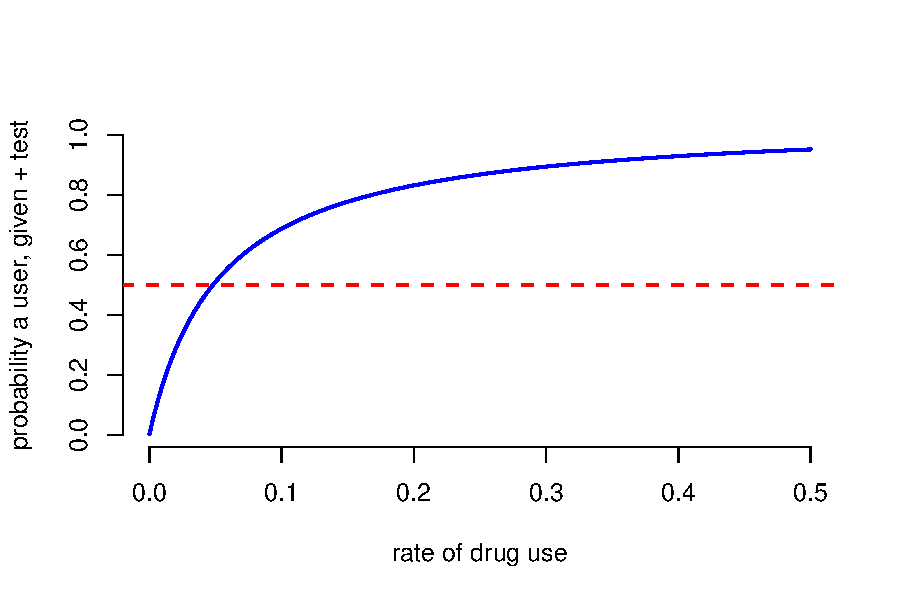
\includegraphics[scale=0.55,trim=10 10 0 50]{drugtest}
\end{center}

Folks often forget this. It's known as the {\rd Base Rate Fallacy}, and is related to the {\rd Prosecutor's Fallacy}.

\end{frame}

\begin{frame}
\chap{Random Variables (RVs)}

A random variable is a variable whose value is subject to randomness. Its possible values and their probabilities are described by a probability distribution. They come in two varieties

\begin{itemize}
\item discrete (numbers of items or successes)
\item continuous (heights, times, weights)
\end{itemize}

\end{frame}


\begin{frame}
\chap{Some Notation}

\begin{itemize}
\item $X$, $Y$ - capital, sometimes bold or with subscripts - RVs
\item $x$, $y$, $k$ - lower case - the values that the RV takes
\item $f(x)$, $f_k$ - functions that return a value for an input $x$ or $k$
\item $\pr(\cdot)$ - ``Probability of $\cdot$''
\item $\E[\cdot]$ - ``the expected value of $\cdot$''
\end{itemize}

\end{frame}


\begin{frame}
\chap{Probability Distributions}

A {\bl Probability Distribution} is a ``is a mathematical description of a random phenomenon in terms of the probabilities of events.'' (Wikipedia)

\sk
That is, it's a mathematical function that gives the probabilities of an RV taking on various alternative values. 

\end{frame}



\begin{frame}
\chap{Discrete RVs}

For discrete RVs, the distribution of probabilities is described by the {\bl probability mass function} (pmf), $f_k$ such that:
\begin{align*}
f_k  \equiv \pr(X & = k) \\
\text{where } 0\leq f_k \leq 1 & \text{ and } \sum_k f_k = 1
\end{align*}
\nsk

For example, for a fair 6-sided die:

$f_k = 1/6$ for $k= \{1,2,3,4,5,6\}$

\end{frame}

\begin{frame}
\chap{Discrete RVs}

Related to the PMF is the {\bl cumulative distribution function} (cdf), $F(x)$. 
\begin{align*}
F(x) \equiv \pr(X \leq x)
\end{align*}
For the 6-sided die
\nsk
\begin{align*}
F(x)= \sum_{k=1}^x f_k
\end{align*}
where $x \in 1\dots 6$.  \\

\end{frame}


\begin{frame}
\chap{Discrete RVs}

Example: RV can take values 1 through 10, each with probability 0.1:

\begin{center}
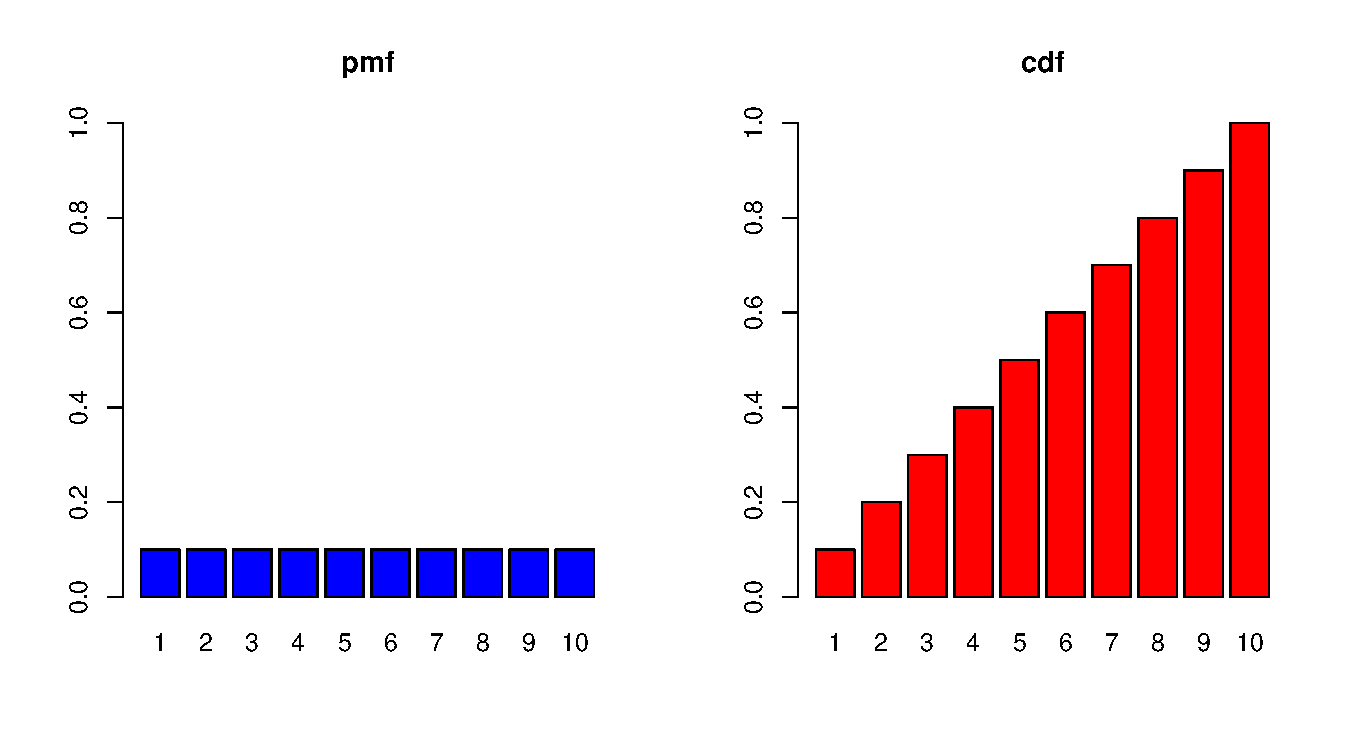
\includegraphics[scale=0.4,trim=10 20 0 10]{discreteRVs}
\end{center}

\end{frame}

\begin{frame}
\chap{Discrete RVs: Practice}

For a fair 6-sided die:

\begin{enumerate}
\item What is $f_k$ if $k=7$? $k=1.5$?
\item What is $F(3)$?  $F(7)$? $F(1.5)$?
\end{enumerate}

\end{frame}


\begin{frame}
\chap{Continuous RVs}

Things are just a little different for continuous RVs. Instead we use the {\bl probability density function} (pdf) of the RV, and denoted by $f(x)$. It still describes how relatively likely are alternative values of an RV, but does not return a probability.

\end{frame}

\begin{frame}
\chap{Continuous RVs}

An analogy:\\
\sk
Probabilities are like {\bl weights}. The PMF tells you how much weight each possible value or outcome contributes to a whole. The PDF just tells you how dense it is around a value. To calculate the weight, you need to also know the size of the area that you're interested in. 

\end{frame}


\begin{frame}
\chap{Continous RVs}

Related to the pdf is the {\bl cumulative distribution function} (cdf), $F(x)$. 
\begin{align*}
F(x) \equiv \pr(X \leq x)
\end{align*}
For a continuous distribution
\nsk
\begin{align*}
F(x)= \int_{-\infty}^x f(x')dx'
\end{align*}

For a normal distribution with mean 0, what is $F(0)$? 

\end{frame}


\begin{frame}
\chap{Continuous RVs}

Example: exponential RV, where $f(x) = re^{-rx}$:

\begin{center}
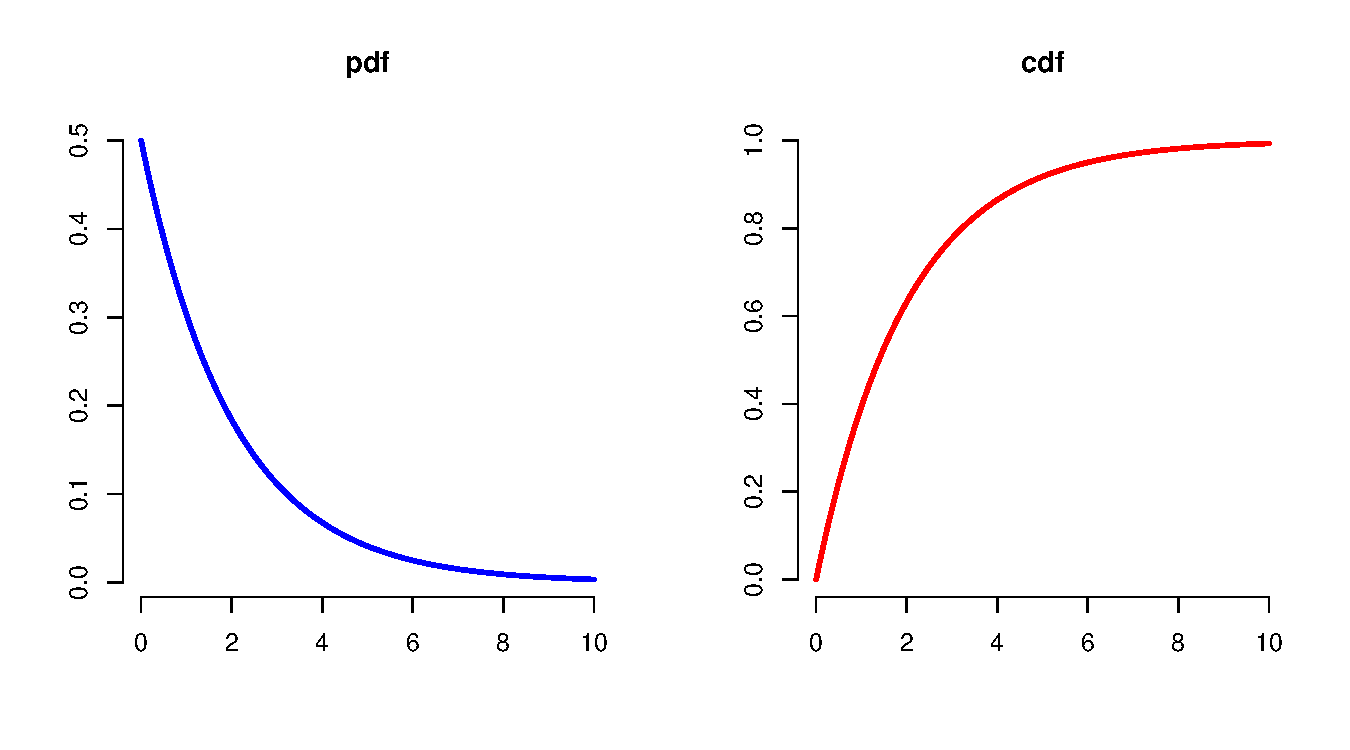
\includegraphics[scale=0.4,trim=10 20 0 10]{continuousRVs}
\end{center}

\end{frame}
%
%\begin{frame}
%\chap{Review summary stats (in {\sf R}) using {\tt swirl}}
%
%We will install another {\tt swirl} lesson to review some moments, and see how to calculate them in {\sf R}. 
%\begin{itemize}
%\item Install the Data Analysis course, following the directions from last time.
%\item Do the ``Central Tendency'' and ''Dispersion'' modules (but don't watch the videos). 
%\end{itemize}
%
%\end{frame}
%


\begin{frame}
\chap{Moments of a RV}

The probability distribution of a random variable can usually be characterized by a small number of parameters, called ``moments''. These are usually defined as:
\begin{align*}
\mu'_n = \E[(X-c)^n] = \int_{-\infty}^{\infty} (x-c)^n f(x) dx
\end{align*}
Here $c$ is some value, and $\E[\cdot]$ is read as ``the expected value of $\cdot$''.  These moments give you lots of information about the distribution -- and you have worked some of them before\dots
\end{frame}


\begin{frame}
\chap{First moment: {\bf mean} }

The expected value (mean), denoted $\mu$ or $\E[X]$  of an R.V. is given by the first moment:
\begin{align*}
\E[X] = \int x f(x) dx \text{\hspace{0.75cm}(continuous RVs)}\\
& \\
\E[X] = \sum_x x f_x \text{\hspace{2cm}(discrete RVs)}
\end{align*}
This moment is the main descriptor of the central tendency or location of your RV. \\
\sk
{\tiny The summation notation/integral is a fancy way of writing down an arithmetic mean of the distribution.}

\end{frame}


\begin{frame}
\chap{Discrete RVs: mean}

Recall, for a fair 6-sided die:

$f_k = 1/6$ for $k= \{1,2,3,4,5,6\}$

\sk
What is $\E[k]$?
\begin{align*}
\E[k] & = \sum_k k f_k  = \sum_{k=1}^{6} k \frac{1}{6}\\
& = \frac{1}{6}  \sum_{k=1}^{6} k = \frac{1}{6} (1+2+3+4+5+6)
\end{align*}
It's like we rolled 6 die and got one of each number - a normal average where the data are perfectly proportioned according to the relative probabilities of outcomes.

\end{frame}



\begin{frame}
\chap{Second moment: variance}

The second {\bl central} moment (i.e., around the mean) is the variance, denoted $\sigma^2$ or $\var(X)$
\begin{align*}
\var(X) & = \E[(X-\mu)^2] = \int (x-\mu)^2 f(x) dx \text{\hspace{0.5cm}(continuous RVs)}\\
&\\
\var(X) & = \E[(X-\mu)^2] = \sum_x (x-\mu)^2 f_x \text{\hspace{1.75cm}(discrete RVs)}
\end{align*}
This moment is a descriptor of variability that is independent of translation (i.e., if you move the mean). 

\end{frame}


\begin{frame}
\chap{Second moment: variance}

Variances are convenient to work with because if $X$ and $Y$ are uncorrelated then $\var(X+Y)=\var(X)+\var(Y)$. However, the variance has units of the mean$^2$, which makes it hard to compare to the mean. There are two common solutions:
\begin{align*}
\sigma = \mr{sd}(X) & = \sqrt{\var(X)}  \text{ \hspace{1cm} standard deviation} \\
& \\
\mr{CV}(X) & = \frac{\sigma}{\mu} \text{\hspace{1cm} coefficient of variation}
\end{align*}

\end{frame}

\begin{frame}
\nochap

{\bf Probability distributions and their moments are descriptors of what we think a {\rd Population} is like.}

\sk
If you know the parameters of the distribution you know everything about the population -- moments, how likely are you to see some values than others, etc. You can calculate a lot of quantities yourself, or you can look things up, or use {\sf R}. 

\end{frame}

\iffalse
\begin{frame}
\chap{Probability Distributions}

In pairs, go onto wikipedia, and look up details of an assigned distribution on Wikipedia. Take note about if it's continuous/discrete, what type of data it usually describes, what it looks like, parameters, $\E[X]$, \var(X), etc. Be ready to split up and tell others in class about your distributions. 
{\small
\begin{itemize}
\item Bernoulli
\item Binomial
\item Poisson
\item Exponential
\item Gamma
\item Beta
\end{itemize}
}

\end{frame}


\begin{frame}
\chap{Second moment: variance}

{\bl Exercise 2.1:} Given that
\begin{align*}
 \E[X+Y]  & = \E[X] + \E[Y]  \text{ \hspace{0.25cm} and \hspace{0.25cm} }  \E[cX]  = c\E[X] \\
\end{align*}
show that
\nsk
\begin{align*}
 \E[(X-\mu)^2]  = \E[X^2] - (\E[X])^2
\end{align*}
\end{frame}
\fi

\begin{frame}[fragile]
\chap{Probability Distributions in {\sf R}}

For standard probability distributions \sf{R} can take random draws, calculate the cumulative distribution, probability density, and quantiles. For the normal distribution:

{\bl
\begin{verbatim}
> rnorm(3, mean=0, sd=1) ## random draws
[1]  0.010666837 -1.518043592 -0.106643773  
> qnorm(p=c(0.025, 0.975), mean=0, sd=1) ## quantiles
[1] -1.959964  1.959964
> pnorm(q=0, mean=0, sd=1) ## cdf, Pr(x<0.5)
[1] 0.5
\end{verbatim}
}

\end{frame}

\begin{frame}[fragile]
\chap{Probability Distributions in {\sf R}}

\nsk
{\bl
\begin{verbatim}
> Y <- rnorm(1000, mean=0, sd=1) 
> hist(Y, freq=F, ylim=c(0, 0.4), 
   xlim=c(-4, 4), main="")
> x<-seq(-10, 10, length=1000)
> lines(x, dnorm(x, mean=0, sd=1), col="red", lwd=2) 
\end{verbatim}
}

\begin{center}
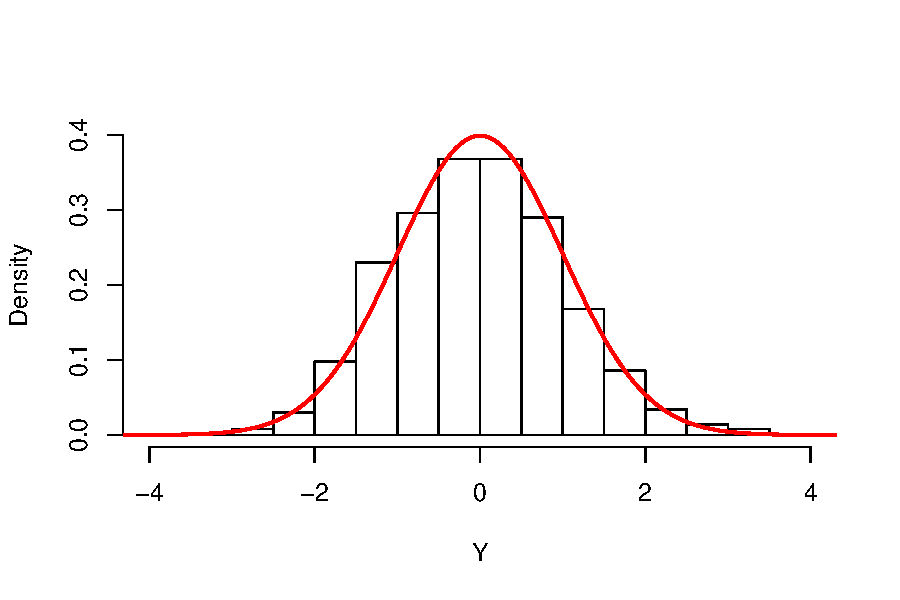
\includegraphics[scale=0.45,trim=10 40 0 40]{norm_dist}
\end{center}

\end{frame}



\begin{frame}
\chap{Normal Distribution}

For the purposes of this course, the {\bl Normal} (or Gaussian) distribution is the most important. Its pdf is:
\begin{align*}
\frac{1}{\sqrt{2\pi}\sigma}\exp{\left(-\frac{(x-\mu)^2}{2\sigma^2}\right)}
\end{align*}
with $\E[x]=\mu$ and $\var(x)=\sigma^2$. Thus the mean and variance are independent. Consider two independent, normally distributed RVs, $X \sim \mN( \mu_x ,\sigma_x^2)$ and $Y \sim \mN( \mu_y ,\sigma_y^2)$. 

\begin{itemize}
\item $cX \sim \mN( c \mu_x , c^2 \sigma_x^2)$
\item $X+b \sim \mN( \mu_x + b , \sigma_x^2)$
\item $X + Y  \sim \mN( \mu_x + \mu_y ,\sigma_x^2 + \sigma_y^2)$
\end{itemize}



\end{frame}



\begin{frame}
\chap{Distribution of the sample mean} 

\sk
Consider
the mean for an $iid$ sample of $n$
observations of a  random variable
$\{X_1,\ldots,X_n\}$.

\sk 
Suppose that $\ds{E}(X_i)  = \mu$ and $\var(X_i) = \sigma^2$, then
\sk
\begin{itemize}
\item $\ds{E}(\bar{X}) = \frac{1}{n} \sum\ds{E}(X_i) = \mu$
\item $\var(\bar{X}) = \var\left( \frac{1}{n} \sum X_i \right) 
=  \frac{1}{n^2} \sum \var\left(  X_i \right) = \displaystyle
\frac{\sigma^2}{n}$.
\end{itemize}

\sk{\bl  If $X$ is normal, then $\bar{X} \sim \mN\left( \mu ,
  \frac{\sigma^2}{n} \right)$. }

\end{frame}

\iffalse

\begin{frame}
\chap{Central Limit Theorem}

What about if $X$ is not normal?
\begin{itemize}
\item {\rd We have the central limit theorem (CLT)! }
\end{itemize}

\sk
The CLT states that for $iid$ random
variables, $X$, with mean $\mu$ and variance $\sigma^2$,
the distribution of the sample mean 
becomes normal as the number of
observations, $n$, gets large. 

\sk That is, {\rd $\displaystyle \bar{X} \rightarrow_{n}
\mN(\mu, \sigma^2/n)$} , and sample averages tend to be
normally distributed in large samples.
\end{frame}

\begin{frame}[fragile]
\nochap

{\bl For example ...} exponential RVs don't look very normal.

{\bl
\begin{verbatim}
x <- seq(0, 5, length=1000)
plot(x, dexp(x), type="l", lwd=2, col="blue")
\end{verbatim}
}

\begin{center}
\includegraphics[scale=0.55,trim=10 10 0 50]{exp_new}
\end{center}

\end{frame}


\begin{frame}
\nochap
{\bl But} if we take lots of samples from the exponential, the distributions of the {\bf mean} do:
\vspace{-0.25cm}
\begin{center}
\begin{tabular}{c c c}
$n=2$ & &$n=10$ \\
\fbox{\includegraphics[height=1in]{exp_2}} & &
\fbox{\includegraphics[height=1in]{exp_10}} \\
& \\
$n=100$ & & $n=1000$ \\
\fbox{\includegraphics[height=1in]{exp_100}} & &
\fbox{\includegraphics[height=1in]{exp_1000}}\\ 
\end{tabular}
\end{center}

\end{frame}

%\addtocounter{page}{-1}
%\begin{frame}
%\nochap
%%\includegraphics[scale=0.6]{exp_2}
%
%\begin{center}
%\includegraphics[scale=0.6]{exp_5}
%\end{center}
%
%\end{frame}
%
%\addtocounter{page}{-1}
%\begin{frame}
%\nochap
%
%\begin{center}
%\includegraphics[scale=0.6]{exp_10}
%\end{center}
%
%\end{frame}
%
%\addtocounter{page}{-1}
%\begin{frame}
%\nochap
%
%\begin{center}
%\includegraphics[scale=0.6]{exp_100}
%\end{center}
%
%\end{frame}
%
%\addtocounter{page}{-1}
%\begin{frame}
%\nochap
%
%\begin{center}
%\includegraphics[scale=0.6]{exp_1000}
%\end{center}
%
%\end{frame}


\begin{frame}
\chap{Normal and Student-$t$}

Recall what {\it Student} (William Sealy Gosset) discovered:

\sk{\rd If $\theta \sim \mN(\mu,\sigma^2)$, but you estimate $\sigma^2
\approx s^2$ based on $n-p$ degrees of freedom, then $\theta \sim
t_{n-p}(\mu, s^2)$.}

\sk The $t$ distribution is just a \bl fat-tailed \bk version of the
normal.  
\begin{itemize}
\item As $n-p \longrightarrow \infty$, our tails get skinny and the
$t$ becomes normal.
\end{itemize}

\end{frame}


\begin{frame}
\nochap

It is usually convenient to work with standardized quantities. 

\[
\frac{\mu - \bar{\theta}}{\sigma} \sim N(0,1) \;\;\; {\bl \Longrightarrow} \;\;\;
{\rd \frac{\mu - \bar{\theta}}{s} \sim t_{n-2}(0,1)} 
\]
Notice that the $t$ and normal distributions from the previous slide, 
and the standardized statistics above, depend upon assumed values for
$\mu$:
\begin{itemize}
\item {\bl  this forms the basis for confidence intervals,
hypothesis testing, and $p$-values.}
\end{itemize}

\sk ---\\
{\small In what follows we will use $Z \sim N(0,1)$ and $Z_{n-p} \sim
t_{n-p}(0,1)$ to represent standardized random variables from normal and
Student-$t$ distributions, respectively.}

\end{frame}


\begin{frame}
\nochap

Suppose $Z_{n-p} \sim t_{n-p}(0,1)$.  A centered interval is\\
\nsk
\[
\rd \mr{Pr}(-t_{n-p,\alpha/2} < Z_{n-p} < t_{n-p,\alpha/2}) = 1-\alpha
\]
\nsk

\begin{center}
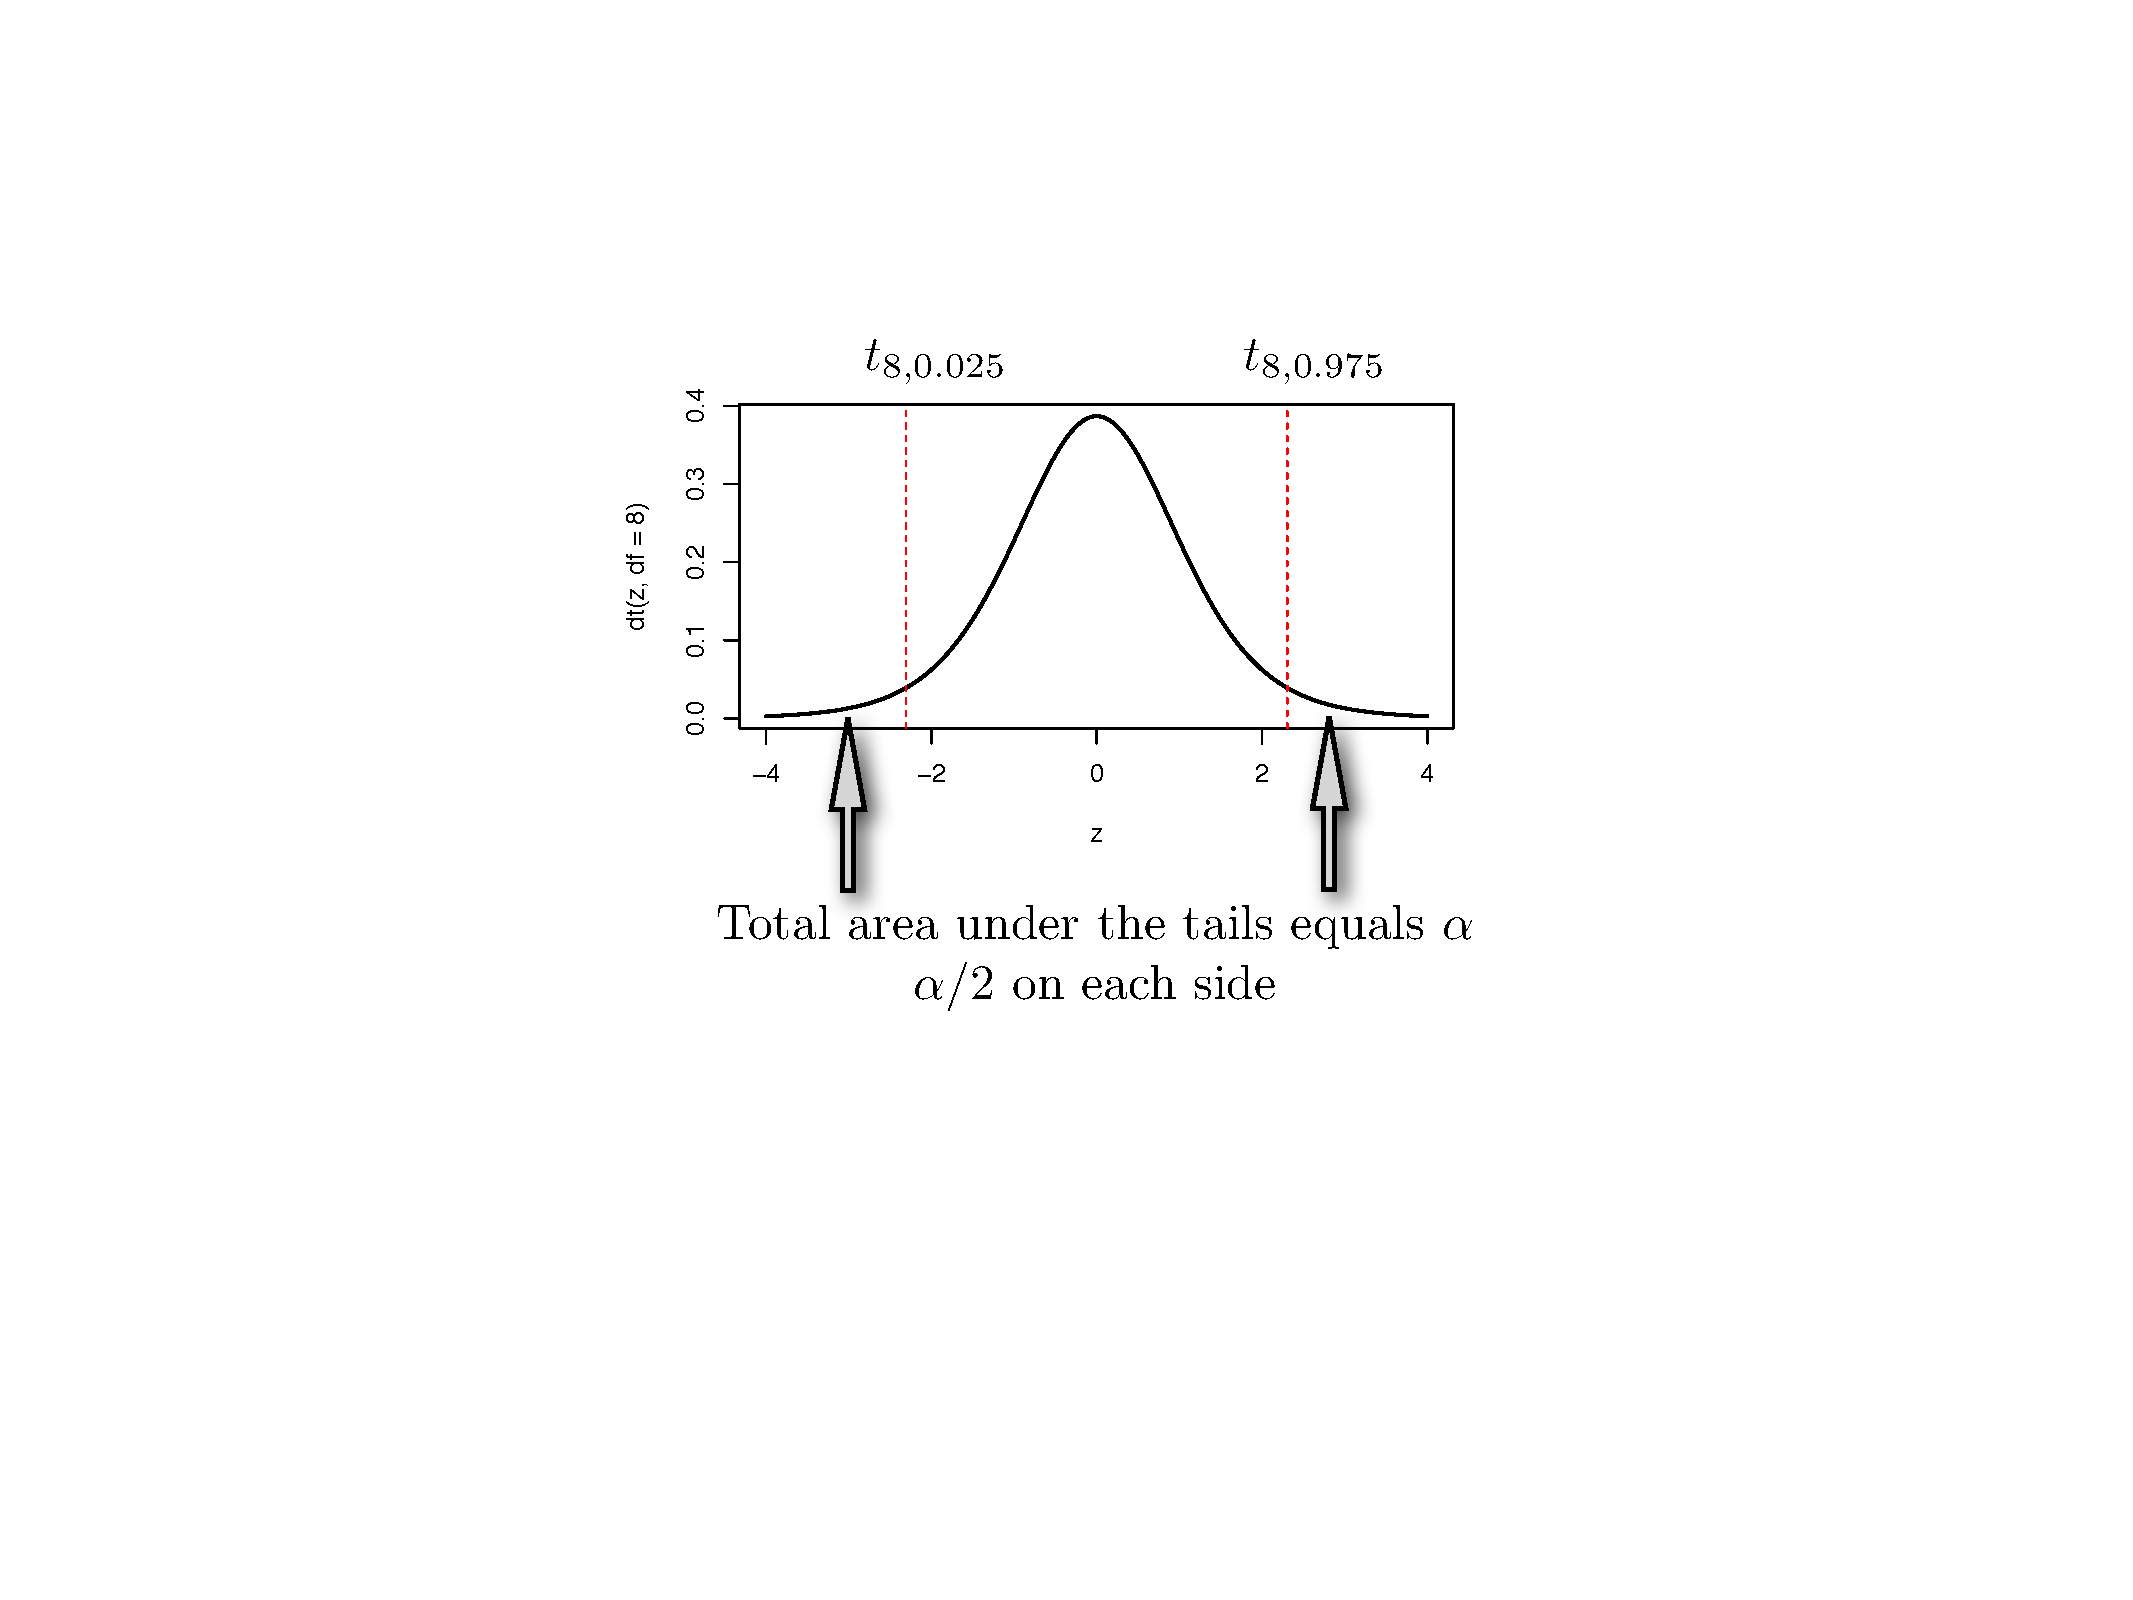
\includegraphics[scale=0.55,trim=20 0 0 15]{tails_new}
\end{center}
\end{frame}

\begin{frame}
\chap{Confidence intervals}

\sk
Since $\theta \sim t_{n-p}(\mu, s^2)$, 
\begin{eqnarray*}
1-\alpha& = &\mr{P}\left(-t_{n-p,\alpha/2} < \frac{\mu - \bar{\theta}}{s} <
t_{n-p,\alpha/2}\right) \\
&=&
\mr{P}(\bar{\theta}-t_{n-p,\alpha/2}s < \mu <
\bar{\theta} + t_{n-p,\alpha/2}s) 
\end{eqnarray*}

\sk
{\bl Thus $(1-\alpha)${\small *100\%} of the time, $\mu$ is
within the confidence interval:} {\rd $\displaystyle
\bar{\theta} \pm t_{n-p,\alpha/2} s$}


\end{frame}



\begin{frame}
\nochap

\nsk\nsk\nsk
\[
 {\bl \bar{\theta} \pm t_{n-p,\alpha/2} s} \;\;\;\;\; \Leftrightarrow \;\;\;\;\; 
{\rd [\bar{\theta}- t_{n-p,\alpha/2} s, \bar{\theta} + t_{n-p,\alpha/2} s] }
\]

\sk
Why should we care about confidence intervals?

\begin{itemize}
\item The confidence interval captures the amount of information 
in the data about the parameter.
\item The center of the interval tells you what your estimate is.
\item The length of the interval tells you how sure you 
are about your estimate.
\end{itemize}

\sk
---\\
{\small  {\tt\rd qt} is the Student-$t$ ``quantile function'', and
 {\tt\rd  qt(alpha, df)} returns $z$ such that 
 {\rd$\alpha = P(Z_{\mathrm{df}} < z)$}}, i.e., {\rd $t_{\mathrm{df},\alpha}$}
\end{frame}


\begin{frame}
\chap{p-Values}

{\bl ``Informally, a p-value is the probability under a specified statistical
model that a statistical summary of the data (e.g., the sample
mean difference between two compared groups) would be equal
to or more extreme than its observed value.''} 
\begin{flushright} 
{\footnotesize ASA Statement on Statistical Significance and P-Values.}
\end{flushright}

\end{frame}


\begin{frame}
\chap{p-Values}

{\bl ``Informally, a p-value is the probability under a specified statistical
model that a statistical summary of the data (e.g., the sample
mean difference between two compared groups) would be equal
to or more extreme than its observed value.''} 
\begin{flushright} 
{\footnotesize ASA Statement on Statistical Significance and P-Values.}
\end{flushright}
\sk
\begin{center}
Hack your own p-values: {\bl \tt \url{http://shinyapps.org/apps/p-hacker/}}
\end{center}

\end{frame}
\fi

\begin{frame}
\chap{Method of Moments}

Consider an $iid$ sample of $n$ observations of a  random variable
$\{x_1,\ldots,x_n\}$. You can calculate sample values of the moments of the RV from these, i.e.:
\nsk
\begin{align*}
\bar{x} & =\frac{1}{n} \sum_{i=1}^n x_i \\
s^2 & = \frac{1}{n} \sum (x-\bar{x})^2
\end{align*}

Then you can estimate the parameters of a probability distribution by ``matching'' these up with the theoretical values of the moments calculated above. This approach can be biased, so it's good to follow up with a maximum likelihood estimate.

\end{frame}

\iffalse
\begin{frame}
%\chap{Probability Distributions: discrete}
\nochap
{\bl Exercise 1: Binomial distribution}\\
{\scriptsize
Used to model the number of ``successes'' in a set of trials (e.g., number of heads when you flip a coin $N$ times). The pmf is 
\begin{align*}
{N \choose x} p^x(1-p)^{N-x}
\end{align*}
such that $\E[x]=Np$ (i.e., this is the theoretical mean). Imagine flipping 20 coins, so that $N=20$.
\begin{enumerate}
\item Take 50 draws from a binomial ({\bl \tt rbinom}) for one of $p\in $ 0.1, 0.5, 0.8 with $N=20$. Plot a histogram of how many successes (out of 20) you got for each of your 50 trials.
\item Calculate the method of moments (MoM) estimate for your? (hint: use the {\tt mean()} function) Is it close to the real value of $p$?
\item For the same value of $p$ take 30 draws from the binomial with $N=20$, and calculate the MoM estimator. Repeat 100 times, and make a histogram. (hint: {\tt replicate()} and {\tt lapply} may be useful.) Is the MoM successfully estimating $p$?
\end{enumerate}
}
%\sk
%{\rd Add hw exercise to calculate the mean and variance of Binom disturb.}

\end{frame}
\fi

\begin{frame}
\nochap
{\bl Exercise 1: Gamma distribution}\\
{\scriptsize
This is the distribution of waiting times until a certain number of events take place. For instance a Gamma(shape=3, scale=2) tells you the distribution of the length of time, in days, you would wait for 3 deaths if the average survival time is 2 days. The pdf is 
\begin{align*}
\frac{1}{s^a\Gamma(a)}x^{a-1}e^{-x/s}
\end{align*}
where $a$ is the shape and $s$ is the scale, $\E[x]=as$ and $\var(x)=(as^2)$. 
\begin{enumerate}
\item Take 20 draws from a gamma ({\bl \tt rgamma}) with $a=3$ and $s=2$, and plot the histogram of samples and overlay the pdf.
\item What are the MoM estimates for $a$ and $s$?
\item Again take 20 draws from the gamma, and calculate the MoM estimates. Repeat 100 times. (hint: {\tt replicate()} or {\tt lapply} may be useful.) Plot histograms of your MoM for each parameter individually as well as jointly on a scatter plot. Indicate the true parameter values in your plots. How does the MoM perform?
\end{enumerate}
}

\end{frame}



\begin{frame}
\chap{Likelihoods}

Recall that $f(Y_i)$ is the pmf (pdf), and it tells us the probability (density) of some yet to be observed datum $Y_i$ given a probability distribution and its parameters. If we make many observations, $\mb{Y}=y_1, y_2, \dots, y_n$, we are interested how probable it was that we obtained these data, jointly. We call this the ``likelihood'' of the data, and denote it as 
\begin{align*}
\mL(\theta; Y)=f_\theta(Y)
\end{align*}
where $f_\theta(Y)$ is the pdf (or pmt) of the data interpreted as a function of $\theta$. 

\end{frame}


\begin{frame}
\chap{Likelihoods}

For instance, for binomial data:
\begin{align*}
\pr(Y_i=k | \theta=p_k)=  {N \choose k} p_k^k(1-p_k)^{N-k}.
\end{align*}
If we have data  $\mb{Y}=y_1, y_2, \dots, y_n$ that are i.i.d. as binomial RVs, the probabilities multiply, and the likelihood is:
\begin{align*}
\mL(\theta; Y) = \prod_{i=1}^n {N \choose y_i} p^y_i(1-p)^{N-y_i}.
\end{align*}


\end{frame}




\begin{frame}
\chap{Likelihoods vs.~probability}

``Likelihood is the hypothetical probability [density] that an event that has already occurred would yield a specific outcome. The concept differs from that of a probability in that a probability refers to the occurrence of future events, while a likelihood refers to past events with known outcomes.'' (1) \\
\sk
Further, the likelihood is a function of $\theta$ (the parameters), assuming fixed data. 


\sk
 ---\\
 {\tiny 1. Weisstein, Eric W. ``Likelihood.'' From MathWorld--A Wolfram Web Resource. {\tt http://mathworld.wolfram.com/Likelihood.html} }

\end{frame}



\begin{frame}
\chap{Likelihoods}

We are usually interested in relative likelihoods -- e.g., is it more likely that the data we observed came from a distribution with parameters $\theta_1$ or $\theta_2$? Thus we only worry about the likelihood up to a constant. Further, it is often easier to work with the log-likelihood:
\begin{align*}
L(\theta; Y) = \ell(\theta; Y) = \log(\mL(\theta;Y))
\end{align*}
where $\log(\cdot)$ is the natural log. 

\end{frame}


\begin{frame}
\chap{Maximum Likelihood Estimators (MLEs)}

We can find the parameters that are most likely to have generated our data -- the maximum likelihood estimate (mle) of the parameters. To do this we maximize the likelihood (or equivalently minimizing the negative log-likelihood) by taking its derivative and setting it equally to zero:
\begin{align*}
\frac{\partial \mL}{\partial\theta_j} =0 \text{\hspace{0.5 cm} or \hspace{0.5 cm}}
-\frac{\partial L}{\partial \theta_j} = 0 
\end{align*}
where $j$ denotes the $j^{\mr{th}}$ parameter. We usually denote the MLE as $\hat{\theta}_j$.
\end{frame}

\begin{frame}
\chap{Likelihoods}

The likelihood {\rd DOES NOT} tell you the probability that parameters have a certain value, given the data. To obtain that quantity, usually called the ``posterior probability of the parameters'' in Bayesian statistics, you have to use Bayes Theorem. 


\end{frame}

\begin{frame}
\nochap

{\bl Exercise 2:}\\

{\footnotesize
Imagine that you flip a coin $N$ times, and then repeat the experiment $n$ times. Thus, you have data $k=k_1, k_2, \dots k_n$ that are the number of times you observed a head in each trial. $p$ is the probability of obtaining a head. 
\begin{enumerate}
\item Write down the likelihood and log-likelihood for the data.
\item Take the derivative of the negative log-likelihood, set this equal to zero and find $\hat{p}$. 
%\item Simulate some data in {\sf R} with $p=0.25$.
%\item Calculate the log-likelihood of your simulated data across a range of $p$ (from 0 to 1), and plot them. This is called a ``likelihood profile''. 
\item If you couldn't fine the MLE analytically, how might you try to estimate it?
\end{enumerate}
}
\end{frame}

\end{document}
